\chapter{Evaluation: Metrics, User Testing, and the Report}
\label{ch:evaluation}

\begin{quote}
\emph{``Without data, you're just another person with an opinion.''} --- Deming. Evaluation turns a demo that \emph{looks} good into evidence that it \emph{is} good---and that you know how to improve it next.
\end{quote}

\noindent\fbox{\parbox{\dimexpr\linewidth-2\fboxsep-2\fboxrule}{%
\textbf{From zero: no prior evaluation training assumed.} We define \emph{metric}, \emph{validity}, \emph{user test}, and \emph{report structure} from first principles with intuition before formality. We assume a built system (Ch.~5) with requirements (Ch.~2) and tests (Ch.~6) to judge it against.}}

\vspace{0.4em}

\section*{Learning Outcomes}
After this chapter you will be able to:
\begin{enumerate}[label=(L\arabic*)]
    \item choose and operationalise metrics (performance, usability, business) linked to success criteria;
    \item design and run a small user study (tasks, consent, think-aloud, SUS) and analyse results honestly;
    \item evaluate requirements coverage, Quality Attributes, and trade-offs with evidence, not adjectives;
    \item write a structured final report (abstract, method, results, threats, conclusion) that audits to the traceability matrix;
    \item identify threats to validity and state limitations without undermining genuine achievement.
\end{enumerate}

% ============================================================
\section{Metrics: Making ``Good'' Measurable}
\label{sec:metrics}

\textbf{Intuition.} ``The system is fast'' convinces nobody. ``p95 latency is 340\,ms at 200 concurrent users, under our 500\,ms NFR'' is verifiable. A \emph{metric} is that translation: an attribute plus a measurement procedure plus a target tied to a requirement ID.

\begin{definition}[Metric and Operationalisation]
A \emph{metric} is a quantitative or categorical measure of a Quality Attribute. \emph{Operationalisation} specifies instrument, procedure, sample, and threshold that turn an abstract goal (``usable'') into a testable claim (``SUS $\ge 75$, $n=8$'').
\end{definition}

Three families cover capstone evaluation:

\begin{itemize}
    \item \textbf{Performance:} latency (p50/p95/p99), throughput (req/s), error rate, resource use (CPU, memory). Measure with load tools (\texttt{k6}, \texttt{JMeter}, \texttt{locust}) on staging that mirrors prod---not your laptop.
    \item \textbf{Usability:} task success rate, time on task, error count, System Usability Scale (SUS), and qualitative observations (think-aloud quotes). Even $n=5$ users find $\sim85$\% of major issues (Nielsen).
    \item \textbf{Business / outcome:} the stakeholder's own success criterion---queue abandonment from 18\% to 9\%, grading time per script from 12\,min to 7\,min---measured before/after or via A/B pilot.
\end{itemize}

Each metric must link \texttt{Req ID} $\to$ \texttt{Metric} $\to$ \texttt{Instrument} $\to$ \texttt{Result} $\to$ \texttt{Verdict}. If a requirement has no metric, it is not evaluable and should be rewritten or descoped.

\begin{figure}[h]
\centering
\begin{tikzpicture}[scale=0.78, every node/.style={font=\scriptsize},
  box/.style={draw,thick,rounded corners=3pt,minimum width=2.0cm,minimum height=0.75cm,align=center},
  arr/.style={-{Stealth[length=2.4mm]},thick,blue!60!black}]
  \node[box,fill=blue!14] (req) at (0,0) {NFR-03\\{\tiny p95 $<$500\,ms}};
  \node[box,fill=green!14] (met) at (3.3,0) {Metric\\{\tiny p95 latency}};
  \node[box,fill=orange!14] (inst) at (6.6,0) {Instrument\\{\tiny k6, 200 VUs}};
  \node[box,fill=violet!14] (res) at (6.6,-1.7) {Result\\{\tiny 340\,ms, 99.1\% pass}};
  \node[box,fill=teal!14] (ver) at (3.3,-1.7) {Verdict\\{\tiny Pass; margin 32\%}};
  \node[box,fill=red!10] (act) at (0,-1.7) {Action\\{\tiny cache if $>$400\,ms}};
  \draw[arr] (req) -- (met); \draw[arr] (met) -- (inst);
  \draw[arr] (inst) -- (res); \draw[arr] (res) -- (ver);
  \draw[arr] (ver) -- (act);
  \draw[arr,dashed,red!60!black] (act) -- (req) node[midway,left,font=\tiny,fill=white] {refine target};
  \node[font=\tiny,gray,align=center] at (3.3,-2.5) {Each arrow is an audit link for the report; missing arrow = unevaluated claim};
\end{tikzpicture}
\caption{Operationalisation chain: requirement becomes metric, metric becomes instrument, instrument yields result and verdict. The dashed feedback refines targets when evidence disagrees with assumptions.}
\label{fig:operationalisation}
\end{figure}

Report metrics with uncertainty: mean $\pm$ SD, confidence interval, or at least min/median/max and sample size $n$. A single run of ``it felt fast'' is anecdote; three runs with variance is evidence. Keep raw data (CSV, logs) in the appendix or repository for reproducibility.

\begin{lstlisting}[language=Python,caption={From raw latencies to a report-ready result: p95 and pass rate with explicit n.},label={lst:metrics-eval}]
import numpy as np

latencies = np.loadtxt("k6_results.csv", delimiter=",")  # ms
p95 = np.percentile(latencies, 95)
pass_rate = (latencies < 500).mean() * 100
print(f"n={len(latencies)}, p95={p95:.0f} ms, pass={pass_rate:.1f}%")
# Verdict: PASS if p95 < 500 and pass_rate >= 99
verdict = "PASS" if (p95 < 500 and pass_rate >= 99) else "FAIL"
print(verdict, "against NFR-03")
\end{lstlisting}

% ============================================================
\section{User Testing: Watching Real People Struggle}
\label{sec:user-testing}

Metrics from machines miss humans. \emph{User testing} watches representative users attempt representative tasks and records where they succeed, hesitate, or fail.

\textbf{Design in 5 steps:} (1)~Define tasks from user stories (``cancel order before acceptance''---not ``click button X''). (2)~Recruit 5--8 participants matching personas, obtain informed consent (purpose, data handling, right to withdraw). (3)~Run think-aloud: ``please say what you are thinking as you go'' with a facilitator who does not help. (4)~Capture: task success (binary), time, errors, SUS questionnaire, and verbatim quotes. (5)~Analyse: affinity diagram observations into themes, prioritise by frequency $\times$ severity.

\begin{figure}[h]
\centering
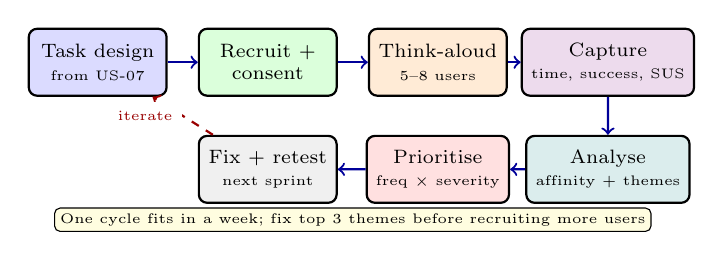
\begin{tikzpicture}[scale=0.80, every node/.style={font=\scriptsize},
  ustep/.style={draw,thick,rounded corners=3pt,minimum width=1.75cm,minimum height=0.85cm,align=center}]
  \node[ustep,fill=blue!14] (t1) at (0,0) {Task design\\{\tiny from US-07}};
  \node[ustep,fill=green!14] (t2) at (2.7,0) {Recruit +\\consent};
  \node[ustep,fill=orange!16] (t3) at (5.4,0) {Think-aloud\\{\tiny 5--8 users}};
  \node[ustep,fill=violet!14] (t4) at (8.1,0) {Capture\\{\tiny time, success, SUS}};
  \node[ustep,fill=teal!14] (t5) at (8.1,-1.7) {Analyse\\{\tiny affinity + themes}};
  \node[ustep,fill=red!12] (t6) at (5.4,-1.7) {Prioritise\\{\tiny freq $\times$ severity}};
  \node[ustep,fill=gray!12] (t7) at (2.7,-1.7) {Fix + retest\\{\tiny next sprint}};
  \draw[->,thick,blue!60!black] (t1) -- (t2); \draw[->,thick,blue!60!black] (t2) -- (t3);
  \draw[->,thick,blue!60!black] (t3) -- (t4); \draw[->,thick,blue!60!black] (t4) -- (t5);
  \draw[->,thick,blue!60!black] (t5) -- (t6); \draw[->,thick,blue!60!black] (t6) -- (t7);
  \draw[->,thick,dashed,red!60!black] (t7) -- (t1) node[midway,left,font=\tiny,fill=white] {iterate};
  \node[font=\tiny,fill=yellow!12,draw,rounded corners=2pt,inner sep=2pt] at (4.05,-2.5) {One cycle fits in a week; fix top 3 themes before recruiting more users};
\end{tikzpicture}
\caption{User-testing loop as a sprint-sized cycle. Each box is a half-day activity; the dashed arrow emphasises iteration---test small, fix, test again beat one big study at the end.}
\label{fig:user-testing-loop}
\end{figure}

\textbf{SUS in 30 seconds.} Ten Likert items (``I would like to use this frequently''), scored 0--100. Above 68 is above average; 75+ is good for capstone. Report mean, range, and $n$---never a single score without context. Pair SUS with qualitative quotes: numbers tell you \emph{how much}, quotes tell you \emph{why}.

\textbf{Ethics and rigour.} Anonymise recordings, store consent forms separately, and allow withdrawal without penalty. For NTU, check whether your study needs IRB review; course-internal usability tests with classmates often qualify for exemption but still require consent. State limitations: sample bias, lab vs.\ field, and instrument validity.

% ============================================================
\section{Interpreting Results: Coverage, Trade-offs, and Threats}
\label{sec:interpreting}

Raw numbers do not speak. Interpretation compares against targets, alternatives, and threats.

{\sloppy \paragraph{Requirements coverage.} Build a table: each Req~ID to test~ID to
metric to result to verdict (Pass/Fail/Partial). Coverage $<100$\% is expected;
explain why the 15\% gap is acceptable (de-scoped Could items with stakeholder
sign-off) rather than hidden. Link to the traceability matrix (Ch.~2) so a marker can audit.\par}

\paragraph{Trade-off analysis.} Every design chooses. Discuss at least two: accuracy vs.\ latency (batch vs.\ streaming inference), security vs.\ usability (2FA friction), completeness vs.\ time-to-market. Show the numbers that forced the choice.

\paragraph{Threats to validity.} Four lenses:
\begin{itemize}
    \item \textbf{Internal:} Did confounds affect results? (Same users before/after; order effects counterbalanced?)
    \item \textbf{External:} Can results generalise? (Lab Wi-Fi vs.\ hawker-centre 4G; student pilot vs.\ full rollout.)
    \item \textbf{Construct:} Does the metric measure the concept? (SUS measures perceived usability, not actual task time.)
    \item \textbf{Conclusion:} Is the sample big enough to claim? ($n=6$ suggests, not proves---report as exploratory.)
\end{itemize}

\begin{table}[h]
\centering\small
\begin{tabular}{@{}lllcc@{}}
\toprule
Req ID & Metric & Instrument & Target & Result \\
\midrule
NFR-03 & p95 latency & k6, 200 VUs, 5\,min & $<500$\,ms & 340\,ms Pass \\
NFR-04 & SUS & 8 users, think-aloud & $\ge 75$ & 78 Pass \\
FR-07  & Cancel success & Gherkin E2E (10 runs) & 100\% & 100\% Pass \\
FR-11  & CSV import 10k & pytest perf & $<1$\,s & 0.82\,s Pass \\
\bottomrule
\end{tabular}
\caption{Example results table: each row audits one requirement to its instrument and verdict. Include $n$ and variance; bold failures and explain them in Discussion.}
\label{tab:results-example}
\end{table}

Honest threats strengthen, not weaken, your report. State each threat, its likely magnitude, and the mitigation you would add with one more sprint.

\paragraph{Reproducibility checklist.} Before submission, verify: raw data committed (CSV/JSON), analysis script reruns with \texttt{python analyse.py} to reproduce every table, seeds fixed, environment pinned (\texttt{requirements.txt}), and anonymised participant data (IDs not names). A reviewer should be able to run \texttt{make eval} and get your numbers.

\begin{example}[Good vs.\ bad evaluation claim]
Bad: ``Users found the system easy to use.'' Good: ``Task~2 (cancel order) success 6/8 (75\%), median time 42\,s (IQR 28--61\,s), SUS mean 78 (SD 8.2, $n=8$), range 65--90. Evidence: k6 run \texttt{results/k6\_run3.csv} and survey \texttt{data/sus\_n8.csv} (commit \texttt{a1b2c3d}). Verdict: NFR-04 Pass; NFR-03 Fail (see Table~\ref{tab:results-example}).'' The second version is auditable in under a minute.
\end{example}

\begin{remark}[Common reporting pitfalls]
Avoid vague adjectives (``fast'', ``intuitive'') without numbers, screenshots without metric callouts, and burying failures in appendices. Put the verdict---Pass or Fail---in the same table as the target so a reader cannot miss it. State effect sizes, not just p-values, when comparing before/after. A useful habit: draft the Results table before running the study, then fill it---this forces you to decide metrics before seeing data.
\end{remark}

\begin{remark}[Appendix hygiene]
List every artefact with a commit hash:
\texttt{data/sus\_n8.csv} and \texttt{k6\_run3.csv} at commit
\texttt{a1b2c3d}, plus consent forms and Gantt snapshots.
If an artefact is not versioned, it does not exist for the marker.
Keep the repository public or provide an anonymous reviewer link.
\end{remark}

% ============================================================
\section{Writing the Report: Structure That Audits}
\label{sec:report}

The report is the persistent evidence that outlives the demo. Structure it so a marker can audit every claim to its source in minutes.

\begin{figure}[h]
\centering
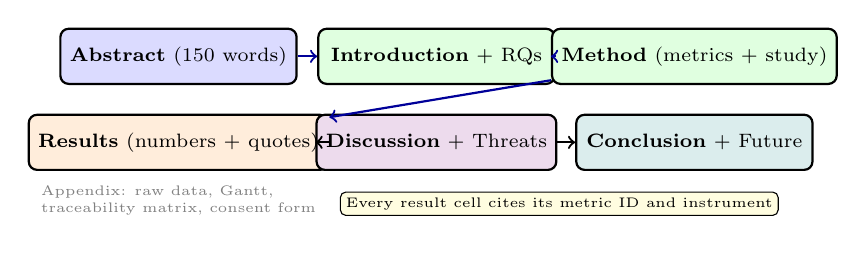
\begin{tikzpicture}[scale=0.78, every node/.style={font=\scriptsize},
  sec/.style={draw,thick,rounded corners=3pt,minimum width=3.0cm,minimum height=0.70cm,align=center}]
  \node[sec,fill=blue!14] (abs) at (0,0) {\textbf{Abstract} (150 words)};
  \node[sec,fill=green!12] (intro) at (4.2,0) {\textbf{Introduction} + RQs};
  \node[sec,fill=green!12] (method) at (8.4,0) {\textbf{Method} (metrics + study)};
  \node[sec,fill=orange!14] (results) at (0,-1.4) {\textbf{Results} (numbers + quotes)};
  \node[sec,fill=violet!14] (discuss) at (4.2,-1.4) {\textbf{Discussion} + Threats};
  \node[sec,fill=teal!14] (concl) at (8.4,-1.4) {\textbf{Conclusion} + Future};
  \draw[->,thick,blue!60!black] (abs) -- (intro); \draw[->,thick,blue!60!black] (intro) -- (method);
  \draw[->,thick,blue!60!black] (method) -- (results); \draw[->,thick] (results) -- (discuss);
  \draw[->,thick] (discuss) -- (concl);
  \node[font=\tiny,gray,align=left] at (0,-2.35) {Appendix: raw data, Gantt,\\traceability matrix, consent form};
  \node[font=\tiny,fill=yellow!12,draw,rounded corners=2pt,inner sep=2pt] at (6.2,-2.4) {Every result cell cites its metric ID and instrument};
\end{tikzpicture}
\caption{Report spine: six sections plus appendix. Colour groups front matter (blue), method/results (green/orange), and synthesis (violet/teal). A marker should be able to trace any sentence in Results back to Method and to a Req ID.}
\label{fig:report-spine}
\end{figure}

Guidance per section: \emph{Abstract}---problem, method, key result, verdict in 150 words. \emph{Introduction}---stakeholder, objectives, success criteria, contribution. \emph{Method}---instruments, participants, procedure (enough to replicate). \emph{Results}---tables of metrics with $n$ and variance; do not interpret yet. \emph{Discussion}---interpret, compare alternatives, and state \emph{threats to validity} (sample size, lab setting, instrument bias). \emph{Conclusion}---what was achieved, what was not, and what you would do with one more sprint. Appendices hold the traceability matrix, raw results, and risk register.

\begin{remark}[One-page evaluation cheat sheet]
Copy this checklist into your report draft: every Req ID has a metric, every metric has an instrument and $n$, every result has a verdict, and every threat has a mitigation. If any cell is blank, the evaluation is incomplete---fill it before writing prose.
\end{remark}

% ============================================================
\section{Exercises}
\label{sec:ch07-exercises}
\begin{enumerate}[label=E7.\arabic*, leftmargin=*, itemsep=0.6em]
    \item \textbf{Operationalise an NFR.} Requirement: ``The dashboard shall feel responsive.'' Rewrite as two testable NFRs (latency + perceived responsiveness), propose metric, instrument, sample size, and pass threshold for each, and sketch the analysis code.
    \item \textbf{User study design.} For ``team formation'' feature, write three tasks, a recruitment plan ($n$, persona, consent line), a think-aloud script, and the data sheet (success, time, errors, SUS). Who would you \emph{exclude} and why?
    \item \textbf{Read a results table.} Given p95 620\,ms ($n=150$, SD 180\,ms) against NFR $<$500\,ms, write the Results sentence and the Discussion paragraph that states the verdict, diagnoses a likely cause (DB N+1), and proposes a fix with expected gain. Do not hide the failure.
    \item \textbf{Threats to validity.} Your study used 6 classmates as participants, all CS majors, in a lab with fast Wi-Fi. List four threats (internal, external, construct, conclusion) and one mitigation per threat you could apply in a second study without extra budget.
    \item \textbf{Report audit.} Take one chapter-2 user story (US-07) and trace it through: Gherkin $\to$ design element $\to$ code module $\to$ test $\to$ metric $\to$ report section. Identify where a missing link would be caught and what artefact must be updated.
\end{enumerate}
% End of Chapter 7
